\section{Applications \& implementation}
\label{sec:implementation}

\begin{figure*}
\label{fig:ihierarchy}
\centering
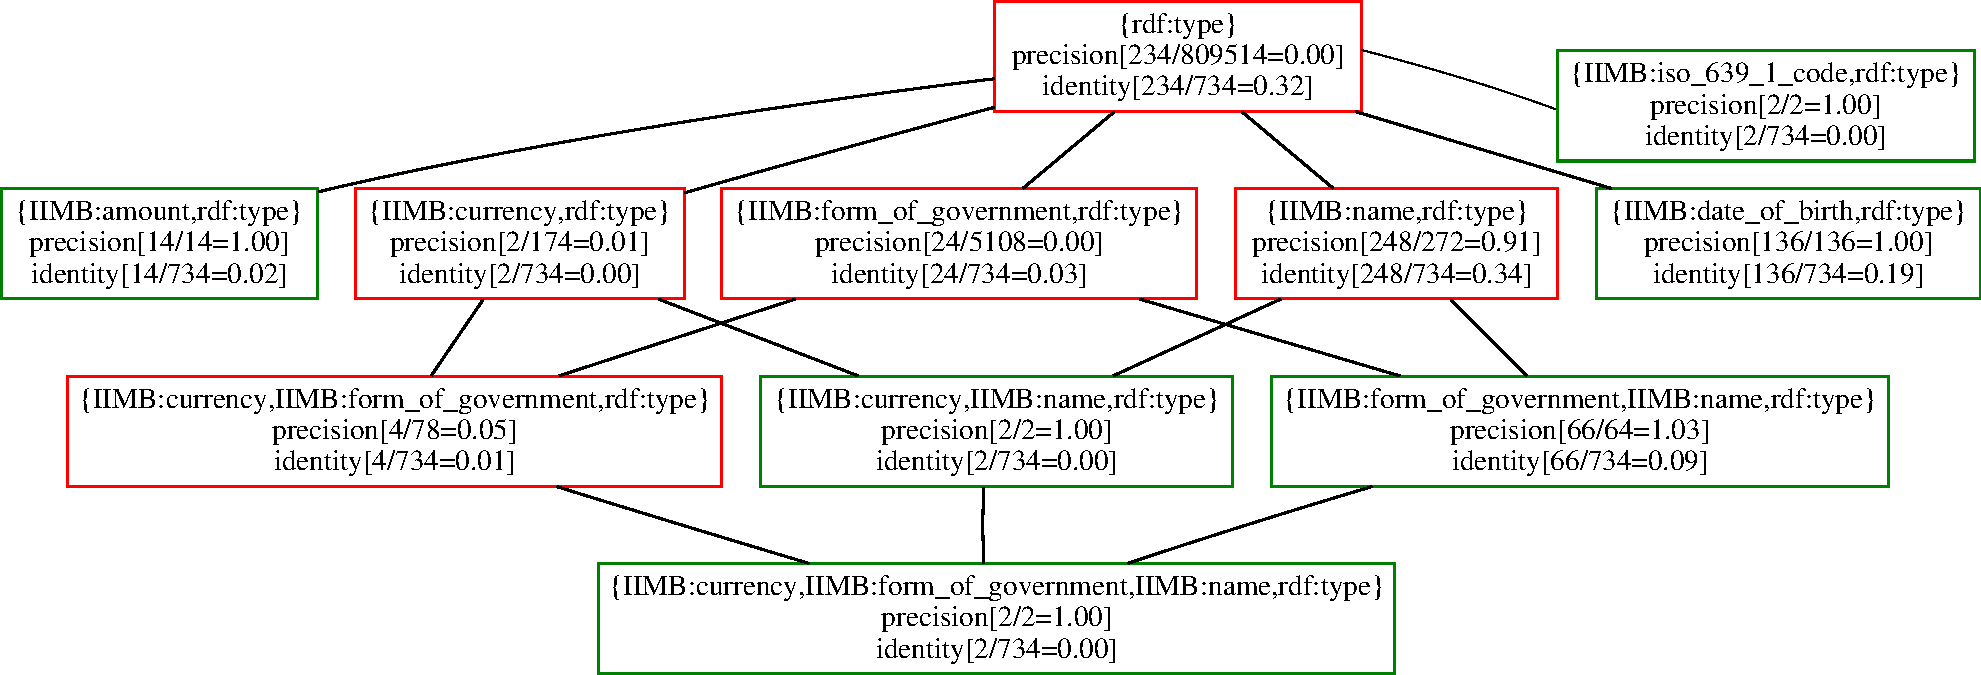
\includegraphics[width=\textwidth]{./img/iimb_16_2}
\caption{
  Example of the identity subrelations for a given dataset (IIMB).
  Each box represents such a subrelation.
  The lower and higher approximation are colored in green and red
    respectively.
  Each box shows the shared predicate terms in curly braces.
  The precision is calculated according to definition \ref{def:precision}.
  The identity figure indicates the number of identity pairs in each box,
    divided by the number of identity pairs overall.
}
\end{figure*}

The approach outlined in section \ref{sec:approach}
  allows us to calculate the subrelation hierarchy of
  a given identity relation.
Figure \ref{fig:ihierarchy} shows an example of the lower and higher
  approximations for a data- and linkset combination of the IIMB database.
Each rectangular box represents an identity subrelation.
Since in this figure a partition is only drawn when there is at least one
  identity pair that is indiscernible with respect to some set of
  predicates, the higher approximation amounts to the entire figure.
The lower approximation only consists of those partition sets that contain
  at least one identity pair, and that contain no non-identity pair;
  these are distinguished by green borders.
For each box the precision is calculated according to
  definition \ref{def:precision}.

\begin{definition}[Precision]
\label{def:precision}
The precision of an identity subrelation is
\[
  \frac{
    \text{The number of identity pairs in the subrelation}
  }{
    \text{The number of pairs in the subrelation}
  }
\]
\end{definition}

\noindent From this definition it is clear that
    subrelations in the lower approximation have precision $1.0$
  and that
    subrelations in the higher approximation have a precision
      between $0.0$ and $1.0$ (exclusive).



\subsection{Applications}
\label{sec:applications}

Based on the partition of the identity relation and the set of all pairs,
  a characterization can be given of the identity relation
  and subrelations can be distinguished (see figure \ref{fig:ihierarchy}).
If we also use the precision of each partition member,
  we can also give suggestions about pairs that may be interesting candidates
  for inclusion in or exclusion from the identity relation.

Alternatively, a low precision may indicate that objects are not
  discernible in terms of the currently asserted predicates.
%This is also a relevant form of feedback,
%  for if a modeler has though of two objects as being identical
%  without them sharing any properties, ...
This often happens when the (natural language) contents of non-typed labels
  are used in order to characterize objects.

Also, the difference between higher and lower approximation
  gives an indication of the quality of the identity relation.



\subsection{Implementation}
\label{sec:implementation}

% INTRO
In order to evaluate our approach outlined in section \ref{sec:approach}
  we implemented an algorithm that calculates
  the discernibility partition, the rough set approximation and
  the quality metric
  for RDF data containing identity statements.\footnote{
      % ALIGNMENT
      Identity statements are either loaded from a VoID-described
        linkset \cite{Void2011}
        or are loaded from an alignment file that are formatted in
        EDOAL (Expressive and Declarative Ontology Alignment Language)
        \cite{DavidEzenatScharffeTrojahn2011}.
    }
The implementation built for this paper is deployed as an extension pack
  of the ClioPatria triple store \URL{cliopatria.swi-prolog.org}.\footnote{
      The code is available at {\small \URL{github.com/wouterbeek/IOTW/}}.
      % PROLOG,GRAPHVIZ,AJAX
      %GraphViz is used for visualizing the hierarchy of
      %  identity subrelations.
      % MATERIALIZATION
      We use Jena 2.11.0 \cite{Carroll2004} in order to materialize
        the graph under RDFS and OWL entailment.
    }

% COMPLEXITY: EASY
Since in real-world data the number of identity pairs
  is relatively small when compared to the number of possible pairs,
  calculating the predicate sets that characterize higher approximation
  subrelations is cheap.
Even calculating this using the path-expressions extension
  (section \ref{sec:path_expressions})
  is cheap, since the number of edge types in RDF data is relatively large;
  so there are not many sequences of identical predicates.
It is also cheap to calculate the predicate sets that characterize
  the lower approximation, plus its extensions,
  since there are relatively few subrelations that belong to it,
  and most such subrelations have a relatively small extension.

% COMPLEXITY: DIFFICULT
It is more costly to calculate the extension of the subrelations that are
  in the higher approximation and that are not in the lower approximation.
This requires an inverse search, starting from sets of
  indiscernibility predicates, and ending with
  -- identical and non-identical --
  pairs of objects sharing all and only those predicates.
The extension of subrelations is, however, necessary in order to
  calculate the quality of the identity relation
  as well as the precision (definition \ref{def:precision})
  of each subrelation.
Since these metrics are useful for the applications outlined
  in section \ref{sec:applications},
  we briefly describe three optimizations.

\textbf{[1] Query optimization.}
Firstly, we optimize the search by restricting the number of pairs
  for which we have to check whether they share a given set of predicates.
We do this by ordering the predicates based on their
  estimated complexity \cite{Wielemaker2005},
  allowing us to match triples that contain rarely occurring predicates
  before matching frequently occurring predicates.
Additionally, by using an arbitrary strict order on terms
  (e.g. lexicographically),
  only half the search space needs to be taken into account
  due to the symmetric nature of equivalence.

\textbf{[2] Datastructures.}
Secondly, we use an AVL tree-based association list
  in order to store the indiscernibility predicates.
The storage of indiscernibility properties uses a similar -- but nested --
  association list mapping sets of predicate terms onto
  sets of subject term pairs.
This means that operations on datastructures are at most $O(\log(n))$.

\textbf{[3] Canonical forms for XML datatypes.}
Thirdly, it is expensive to determine whether lexical expressions
  of the same datatype are identical or not,
  due to time spent on parsing those expressions
  in order to determine their value.
The -- worst case -- number of such parses is quadratic
  in the number of same-typed literals.
Since canonical mappings are one-to-one \cite{XmlSchema2012},
  it is possible to determine value identity by comparing
  canonical lexical expressions,
  requiring only a linear number of lexical expression parses.
This is achieved by converting all lexical expressions
  to their canonical lexical form prior to running the main algorithm.

\begin{comment}
Existing SW libraries implement equivalence relations for common datatypes,
  but equivalence is not always in line with identity.
Therefore, exceptions have to be made for specific values
  that are known to have equivalent non-identities (such as $0$ and $-0$)
  and non-equivalent identities (such as $NaN$ for {\small \texttt{float}}).
The latter even provides a rare instance of violating the common definition
  of identity as the smallest equivalence relation.
\end{comment}
